\documentclass[a4paper,10pt]{article}
\usepackage{fancyvrb}
\usepackage{graphicx}
\graphicspath{ {graficos/} }
\usepackage[ansinew]{inputenc}
\usepackage{float}
\usepackage[colorlinks=true,linkcolor=black,urlcolor=blue,bookmarksopen=true]{hyperref}
\usepackage{bookmark}
\usepackage{fancyhdr}
\usepackage{bbm}

\pagestyle{fancy} % Encabezado y pie de p�gina
\fancyhf{}
\fancyhead[L]{Sebastian Elizade - Julian Ferres}
\fancyhead[R]{Aprendizaje Estad�stico - FIUBA}
\renewcommand{\headrulewidth}{0.4pt}
\fancyfoot[C]{\thepage}
\renewcommand{\footrulewidth}{0.4pt}

\title{ \Huge \textbf{Colecci�n de Ejercicios Propuestos y sus resoluciones\\}}
\author{
	\Huge Sebastian Elizalde
	\\
	\LARGE \textit{Padr�n Nro. 96092}        \\
	\LARGE    \texttt{sebi.elizalde@gmail.com}                                              \\[2.5ex]
	\\
	\Huge Julian Ferres
	\\
	\LARGE \textit{Padr�n Nro. 101483}                     \\
	\LARGE    \texttt{julianferres@gmail.com}                                              \\[2.5ex]
	\LARGE   2do. Cuatrimestre de 2018                                      \\        
	\\
	\LARGE  Aprendizaje Estad�stico - Sebastian Grymberg  \\        
	\\
	\LARGE  Facultad de Ingenier�a, Universidad de Buenos Aires            \\}
\date{}
\begin{document}
	\maketitle
	% quita el n�mero en la primer p�gina
	\thispagestyle{empty}
	\newpage
	\tableofcontents
	\newpage
	\section{Introducci�n}
	

	\section{Lista de enunciados y sus soluciones}
	
	
	
	\subsection{Clase 1}
	
	\subsubsection{Ejercicio 1}
	
	Sea una funci�n convexa $f(x)$ no negativa, $x_0,x_1,x_2$ tales que:
	
	\begin{itemize}
		
		\item $x_1 \leq x_0 \leq x_2$
		
		\item $x_0 = p_1x_1+p_2x_2$ 
		
		\item $p_1 \geq 0 , p_2 \geq 0 , p_1+p_2=1$ 
		
	\end{itemize}
	
	
	Y sea una recta $g$ tal que:
	
	\begin{itemize}
		
		\item $g(x_1) = f(x_1)$
			
		\item $g(x_2) = f(x_2)$
	
	\end{itemize}
	
	
	Quedan dudas de cu�l de los siguientes era el planteo:
	Comprobar la siguiente desigualdad:
	f(p?x?+p?x?) p?f(x?) + p?f(x?) 
	
	Probar que:
	g(x0) = p1 g(x1) + p2 g(x2) 
	
	
	\subsubsection{Ejercicio 2: Esperanza condicional}	
	
	Utilizando que
	$E[m(x) f(x)] = E[Yf(x)]$ y $ m(x)=E[Y|X=x]$\\
	
	Demostrar que vale:
  $E[\Phi(x)Y| X] = \Phi(x)E[Y|X]$
	
	
	\subsubsection{Ejercicio 3 (STOP) (SIMULACI�N)}
	
	Sea $ X \sim \mathcal{N}(0,\, 1)$ truncada al intervalo $\left[-1,1\right]$	
	
	Imagine  $m(x) = E[Y | X=x]$ como:\\
	
	   $
	   m(x) := \left\{
	   \begin{array}{ll}
	   \frac{(x + 2)^2}{2} & \mathrm{si\ } si -1\leq x<-0.5 \\
	   \frac{x}{2}+0.875     & \mathrm{si\ } -0.5 \leq x \leq 0\\
	   -5(x-0.2)^2 +1.075 & \mathrm{si\ } 0 < x \leq 0.5 \\
	   x + 0.125 & \mathrm{si\ } 0.5 \leq x < 1 
	   \end{array}
	   \right.
	   $
	\\

	Dado un $x$, la distribuci�n condicional de $Y - m(x)$ es
	$\mathcal{N}(0,\, \sigma^2(x))$
	
	Con $\sigma(x)=0.2-0.1\cos(2x)$\\
	
	Se pide simular $200$ puntos $(X,Y)$, y graficarlos en un plano. 
	
	Adem�s, se piden los $200$ pares ordenados en cuesti�n, para hacer an�lisis posteriores.
	
	
	\subsubsection{Ejercicio 4 (no entregable)}
	

	Dado el problema de decisi�n introducido en el 'Dise�o del receptor de una comunicaci�n binaria', verificar que:\\ 
	$\delta(r) = \mathbbm{1}\{{ P(S=1 | R=r) > P(S=0 | R = r) }\}$\\ maximiza:\\
	$P(S=\delta(r)) =P(S=\delta(0) | R=0)P(R=0) + P(S=\delta(1) | R=1)P(R=1)$
	
	\subsection{Clase 2}
	
	\subsubsection{Ejercicio 5}
	
	Terminar la cuenta:
	
	$$ P(X,Y) = \int_{0}^{\frac{1}{2}} (1-x) dx + \int_{\frac{1}{2}}^{\frac{3}{4}} x dx $$
	
    \textbf{\underline{Soluci�n:}}
    
    $$ P(X,Y) = \int_{0}^{\frac{1}{2}} (1-x) dx + \int_{\frac{1}{2}}^{\frac{3}{4}} x dx $$
	$$ = \int_{0}^{\frac{1}{2}} 1 dx - \int_{0}^{\frac{1}{2}} x dx + \int_{\frac{1}{2}}^{\frac{3}{4}} x dx $$
	$$ = {\frac{1}{2}} - {\frac{1}{8}} + ({\frac{9}{32}} - {\frac{1}{8}}) $$
	$$ = 17/32 $$
	
	
	\subsubsection{Ejercicio 6}
	
	Sean $T, F$ y $E$ exponenciales de intensidad $1$ y tenemos que 
	
	$$ Y = \mathbbm{1}\{T + F + E < 7\}$$
	
	Se tenia que $E$ era inobservable. Y se concluy� que:
	
	$$ g^*(T,F) = \mathbbm{1}\{ T+ F < 7 - \ln{2}\}$$
	
	Se pide calcular el error:
	
	$$L^* = P ( g*(T,F) \neq Y)$$
	
\textbf{\underline{Soluci�n:}}
	
	$$L^* = P ( g*(T,F) \neq Y) $$
	$$ = P(T + B < 7 - log2 , T + B + E \geq 7) + P(T + B \geq 7 - log2, T + B + E < 7)$$
	$$ = E(e^{-(7-T-B)} \mathbbm{1}\{T + B < 7 - log2\}) + P((1-e^{-(7-T-B)}) \mathbbm{1}\{7 > T + B \geq 7 - log2 \}) $$
	$$ = \int_{0}^{7 - log2} x e^{-x} e^{-(7-x)} dx  + \int_{7-log2}^{7} x e^{-x} (1-e^{-(7-x)}) dx $$
	(porque la densidad de T + B es $ue^{u}$ en $[0,\infty)$)
	$$ = e^{-7} \left({\frac{(7-log2)^2}{2}} + 2(8-log2)-8-{\frac{7^2}{2}} + {\frac{(7-log2)^2}{2}} \right) $$
	(ya que $ \int_{x}^{\infty} u e^{-u} du = (1+x)e^{-x}$ )
	$$ = 0.0199611... $$
	
	
	\subsection{Clase 3}
	
	\subsubsection{Ejercicio 7}
	Se quer�a acotar:\\
	
	$E \left[ | \eta^{*} (x) - \eta(x)| \right]  < \epsilon  $	\\
	
	Para $\epsilon>0$ existe una funci�n $\eta_{\epsilon}$ uniformemente continua a valores en el intervalo $\left[ 0, 1 \right]$ sobre un conjunto compacto $C$ que se anula fuera de $C$, y que tiene la siguiente propiedad:\\
	$E[ |\eta_\epsilon(x) - \eta(x)| ] < \epsilon $ \\
	
	Por la desigualdad triangular:\\
	
	$E\left[ |\eta^*(x) - \eta(x)| \right] \leq E[ |\eta ^*(x) - \eta_\epsilon ^*(x)| ] + E[ |\eta^*_\epsilon(x) - \eta_\epsilon(x)| ] + E[ |\eta_\epsilon(x) - \eta(x)| ]$\\
		
	En clase se acotaron tanto el tercer t�rmino como el segundo del segundo miembro de la desigualdad, y el ejercicio es entender  por qu� el primer t�rmino est� acotado por el tercero.
	
	\subsubsection{Ejercicio 8 (STOP)(SIMULACI�N)}
	
	Dado el siguiente diagrama:
	\begin{center}
	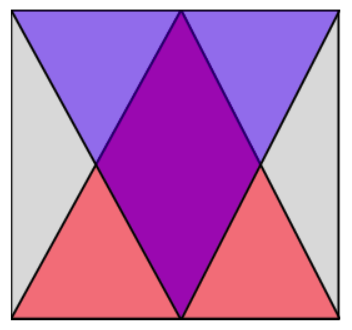
\includegraphics[width=0.5\linewidth]{enunciado-ej8}
	\label{fig:enunciado-ej8}\\
	\end{center}
	
	Sean:\\
	
	$X$ una variable aleatoria con distribuci�n uniforme sobre el triangulo \textbf{azul}.\\
	
	$Y$ una variable aleatoria con distribuci�n uniforme sobre el triangulo \textbf{rojo}.\\
	
	$Z$ se define como: 	
	 $Z = \frac{1}{2}X + \frac{1}{2}Y$\\
	 
	Se pide:
	 
	\begin{enumerate}
	
	\item	Generar muestras de X y de Y para aprender.
	
	\item	Generar muestras a clasificar uniformes sobre el cuadrado completo.
	
	\item	Construir una regla del histograma y clasificar las muestras de 2. seg�n lo aprendido en 1. .
	
	\item	Graficar los resultados.
	
	\end{enumerate}

	\subsection{Clase 4}
				
	\subsubsection{Ejercicio 9: KNN}
	
	
	Se pide simular dos normales bivariadas, ambas con matriz de covarianza $\left[ \left[ 1 , 0 \right] , \left[ 0,1\right] \right]$	
	, pero una centrada en $(-1, 0)$, y la otra en $(1, 0)$.\\
	
	Se pide:
	\begin{enumerate}
	
		\item	Generar muestras de N = 100, 1000, ... , otros valores. Estas dos ser�an las clases en las que clasificar los puntos.
		
		\item 
		Generar puntos con una distribuci�n uniforme en $\left[-4, 4\right] \times \left[-4, 4\right]$.
		
		\item Clasificar los puntos de la uniforme usando $KNN$, con $K = 1, 3$ y $13$, utilizando las clases del primer item.
		
		\item Graficar los resultados.
	\end{enumerate}

	
	
	

	\subsubsection{Ejercicio 9 bis}
	"Redactar una carilla que contenga la informaci�n relevante sobre la distribuci�n normal multivariada. Llevar ejemplos, y mostrar como cambia el gr�fico al variar la matriz de covarianza."
		
	\subsubsection{Ejercicio 10}
	
	Demostrar que $\forall a,b,c \in \mathbbm{R}^+$:
	
	$$ (a+b+c)^2 \leq 3(a^2+b^2+c^2)$$
	
	Sugerencia: usar Cauchy-Schwarz / Jensen.
	
	
	\subsection{Clase 5}
	
	\subsubsection{Ejercicio 11}
	
	Dadas las desigualdades:\\
	
	$$P(S_n - E\left[S_n\right] \geq \epsilon ) \leq e^{-2\epsilon^2/ \sum_{i=1}^{n} (b_i-a_i)^2}$$
	
	$$P(S_n - E\left[S_n\right] \leq -\epsilon ) \leq e^{-2\epsilon^2/ \sum_{i=1}^{n} (b_i-a_i)^2}$$
	
	Probar que se cumple la siguiente desigualdad:\\
	
	
	$$P(|S_n - E\left[S_n\right]| \leq -\epsilon ) \leq 2 e^{-2\epsilon^2/ \sum_{i=1}^{n} (b_i-a_i)^2}$$
	
	Sugerencia: Usar que $P(A \cup B) \leq P(A)+P(B)$
	
	
	\subsubsection{Ejercicio 12}
	En clase se demostr� la primer desigualdad de la hipotesis del ejercicio anterior.\\ Se pide como ejercicio demostrar la segunda desigualdad de la hipotesis.
	
	\subsubsection{Ejercicio 13}
	
	Dada la funci�n:
	
	$$ \Phi(u) = \ln{p e^u +1 -p} - pu$$
	
	Mostrar que:
	
	\begin{itemize}
		\item $\Phi(0) = 0$
		\item $\Phi'(0) = 0$
		
		
	\end{itemize}
	
	\subsubsection{Ejercicio 14 (STOP)}
	
	Dados los siguientes clasificadores por particiones:
	
	\begin{center}
		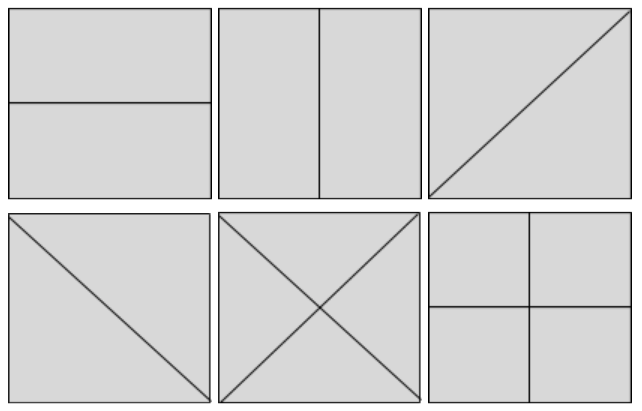
\includegraphics[width=0.5\linewidth]{enunciado-ej14}
		\label{fig:enunciado-ej14}\\
	\end{center}
	
	Elegir cu�l es el mejor para las clases y los puntos generados en el ejercicio 8.
	
	\subsection{Clase 6}
	
	\subsubsection{Ejercicio 15}
	
	Demostrar que la siguiente secuencia constituye una serie convergente:
	
	$$a_n = 8(n+1) e^{-n\epsilon^2/32}$$
	
	Y generalizar viendo que $\forall \lambda >0$:
	
	$$ \sum_{n=0}^{\infty} n e^{-\lambda n} < \infty$$
	
	(Sugerencia: Usar que $\int_{0}^{\infty} xe^{-\lambda x}dx = \frac{1}{\lambda^2}$)
	

	\subsubsection{Ejercicio 16}
	
	Sea la familia de intervalos:
	
	$$ A' =\{ (a,b): a< b \} $$
	
	Luego de calcular $N_{A'}(z_1,z_2) = |\{\emptyset, \{z_1\},\{z_2\},\{z_1,z_2\}\}|= 4$ en clase, se pide calcular:
	
	\begin{enumerate}
		\item $N_{A'} (z_1,z_2,z_3)$
		
		\item $N_{A'} (z_1,z_2,\cdots, z_n)$
	\end{enumerate}
	
	
	\section{Conclusiones}

	\begin{thebibliography}{99}
		\bibitem{}
	\end{thebibliography}
\end{document}
